\documentclass[10pt]{article}
\usepackage[utf8]{inputenc}
%\usepackage{html}
\usepackage{booktabs}
\usepackage{amsmath}
%\usepackage{natbib}
\usepackage{graphicx}
\usepackage{fullpage}
\usepackage{longtable}
\usepackage{float}
%\usepackage[colorlinks=true,urlcolor=blue,linkcolor=blue,menucolor=blue]{hyperref}
\usepackage{hyperref}

%allow column deletion http://tex.stackexchange.com/q/16604/1783
\usepackage{array}
\newcolumntype{H}{>{\setbox0=\hbox\bgroup}c<{\egroup}@{}}

%remove spacing between items in a list
\usepackage{enumitem}
\setlist{labelindent=\parindent,leftmargin=*,itemsep=0pt,parsep=0pt}

%\providecommand{\alert}[1]{\textbf{#1}}
\setcounter{secnumdepth}{2}

%% less conservative float placement
\renewcommand{\topfraction}{.85}
\renewcommand{\bottomfraction}{.7}
\renewcommand{\textfraction}{.15}
\renewcommand{\floatpagefraction}{.66}
\renewcommand{\dbltopfraction}{.66}
\renewcommand{\dblfloatpagefraction}{.66}
\setcounter{topnumber}{9}
\setcounter{bottomnumber}{9}
\setcounter{totalnumber}{20}
\setcounter{dbltopnumber}{9}


\date{}
\title{The Biofuel Ecopysiological Traits and Yields Database:\\ Database Description and User's Guide\\Version 1.0}
\author{David LeBauer, Dan Wang, Patrick Mulrooney, Mike Dietze}
\begin{document}
\maketitle 
% Download this User's Guide as \href{https://netfiles.uiuc.edu/dlebauer/www/dbdocumentation_users.pdf}{PDF}.
% Download the Data Entry Workflow as. 
\vspace{5in}
\noindent \textit{Please cite this document regarding the implementation and structure of BETY:}

David LeBauer, Dan Wang, Patrick Mulrooney, Mike Dietze. 2011. The Biofuel Ecopysiological Traits and Yields Database: Database Description and User’s Guide, Version 1.0
\vspace{1em}

\noindent \textit{Please cite the use of data contained in BETY:}

 David LeBauer, Dan Wang, and Michael Dietze, 2010. Biofuel Ecophysiological Traits and Yields Database Version 1.0. Energy Biosciences Institute, Urbana, IL. \texttt{http://ebi-forecast.igb.uiuc.edu/bety}

\newpage
\tableofcontents
\newpage
\listoftables
\listoffigures

\newpage
\section{Quick Start}
\begin{description}
\item[Open web interface:] \href{http://ebi-forecast.igb.uiuc.edu/bety/}{ebi-forecast.igb.uiuc.edu/bety/}
\item[Download data:] \autoref{sec:download}.
\item[Enter data:] see the \href{https://netfiles.uiuc.edu/dlebauer/www/dbdocumentation_data_entry.pdf}{Data Entry Workflow}.  
\item[Read about table contents:] see \autoref{tab:tables} and \autoref{sec:tables}.
\item[View summary of core tables and relationships : \autoref{fig:summarymodel}]
\item[View comprehensive schema, \autoref{fig:model}].
\end{description}
  
% \subsection{Query BETYdb through web interface}
% Trait and yield data in BETYdb can be queried in multiple ways.  BETYdb can be reached through its web interface \url{http://ebi-forecast.igb.uiuc.edu/ ebi-forecast.igb.uiuc.edu}.


% \begin{description}
% \item[Species] individual species genera can be queried using their genus, species, common name, or USDA Symbol.
% \item[Growth Form] tree, shrub, vine, forbs and herbs, perrenial grass or sedge, and annual grass or sedge.
% \item[Water Demand] xeric (drought tolerant or minimum precipitation $<15$in), hydric (USDA State or Federal Wetland indicator) or mesic (neither mesic nor hydric).
% \item[climate]  (based on minimum temperature) tropical ($>0^o$C), arctic ($<-45^o$C), or temperate (neither arctic nor tropical).
% \end{description}

\section{Background}
 A major motivation of the biofuel industry is to reduce greenhouse gas emissions by providing ecologically and economically sustainable sources of fuel and dependence on fossil fuel.
 The goal of this database is to provide a clearinghouse of existing research on potential biofuel crops, to provide a source of data on plant ecophysiological traits and yields, and to present ecosystem scale re-analysis and forecasts that can support the agronomic, ecological, policy, and economic aspects of the biofuel industry.
 This database will facilitate the scientific advances and assesments that this transition will require.

\section{Introduction}
 This document describes the purpose, design, and use of the Biofuel Ecophysiological Traits and Yields database (BETYdb).
 BETYdb is a database of plant trait and yield data that supports research, forecasting, and decision making associated with the development and production of cellulosic biofuel crops.
 While the content of BETYdb is agronomic, the structure of the database itself is general and can therefore be used more generally for ecosystem studies.
 
  BETY-db can be accessed online at \href{http://ebi-forecast.igb.uiuc.edu/bety/}{ebi-forecast.igb.uiuc.edu/bety/}. 
  For developers interested in the database description in SQL syntax, e.g. to explore, create, and modify its structure, the \href{https://github.com/dlebauer/BETYdb/raw/master/betydb_schema.sql}{betydb\_schema} is available.
 or further information about the proceedures that are used to enter data into the database, see the accmpanying \href{https://netfiles.uiuc.edu/dlebauer/www/dbdocumentation_data_entry.pdf}{Data Entry Workflow}.
 

\subsection{Objectives}

 The objectives of this database are to allow other users access data that has been collected from previously published and ongoing research in a consistent format, and to provide a streamlined interface that allows users to enter their own data.
 These objectives will support specific research and collaboration, advance agricultural practices, and inform policy decisions.
 Specifically, BETYdb supports the following uses:

\begin{enumerate}
\item Carry out statistical analyses to explore the relationships between traits
\item Identify differences among species and functional groups
\item Access BETY-db from simulation models to look up values for traits and parameter
\item Identify gaps in knowledge about biofuel crop traits and model parameters to aid rational planning of research activities
\end{enumerate}

 BETYdb provides a central clearinghouse of biofuel crop physiological traits and yields in a consitently organized framework that simplifies the use of these data for further analysis and interpretation.
 Scientific applications include the development, assessment, and prediction of crop yields and ecosystem services in biofuel agroecosystems. 
 The database directly supports parameterization and validation of ecological, agronomic, engineering, and economic models.
 The initial target end-users of BETY-db version 1.0 are users within EBI who aim to support sustainable biofuel production through statistical analysis and ecological modeling.
 By streamlining the process of data summary, we hope to inspire new scientific perspectives on biofuel crop ecology that are based on a comprehensive evaluation of available knowledge.

 Published data and analyses will be provided to other scientists and the public in an easy to understand, interactive web front end to the database.

\section{Scope}
 The database contains trait, yield, and ecosystem service data.
 Because all plants have the potential to be used as biofuel feedstock, BETYdb supports data from all plant species.
 In practice, the species included in the database reflect available data and the past and present research interests of contributors.
 Trait and yield data are provided at the level of species, with cultivar and clone information provided where available.

 The yield data not only includes end of season harvestable yield, but also includes measurements made over the course of the growing season.
 These yield data are useful in the assessment of historically observed crop yields, and they can also be used in the validation of plant models.
 Yield data includes peak biomass, harvestable biomass, and the biomass of the crop throughout the growing season.

 The trait data represent phenotypic traits; these are measurable characteristics of an organism.
 The primary objective of the trait data is to allow researchers to model second generation biofuel crops such as Miscanthus and Switchgrass. 
 In addition, these data enable evaluation of new plant species as potenial biofuel crops.
 Ecosystem service data reflect ecosystem-level observations, and these data are included in the traits table.

\subsection{Data Content}
 BETYdb includes data obtained through extensive literature review of target species in addition to data collected from the Energy Farm at the  University of Illinois, and by our collaborators. 
 The BETYdb database contains trait and yield data for a wide range of plant species so that it is possible to estimate the distribution of plant traits for broad phylogenetic groups and plant functional types.

 BETYdb contains data from intensive efforts to find data for specific species of interest as well as from previous plant trait and yield syntheses, and other databases.% (Table \ref{tab:externaldata}).
 Most of the data currently in the database is from plant groups that are the focus of our current research (\autoref{tab:internaldata}).
 These species include perennial grasses, such as Miscanthus (\textit{Miscanthus sinensis}) Switchgrass (\textit{Panicum virgatum}), and sugarcane (\textit{Saccharyn} spp.).
 BETY also includes short-rotation woody species, including poplar (\textit{Populus} spp.) and willow (\textit{Salix} spp.) and a group of species that are being evaluated at the energy farm as novel woody crops.
 In addition to these herbaceous species, we are collecting data from a species in an experimental low-input, high diversity prairie. 

\begin{table}[hbt]
  \begin{tabular}{lcc}
    \hline
    \textbf{Genus} & \textbf{Traits} & \textbf{Yields} \\ 
    \hline \hline
    Miscanthus	&2741	&506\\
    Populus	&1740	&755\\
    Panicum	&606	&1904\\
    Salix	&146	&136\\
    Andropogon	&92	&\\
    Agave	&88	&\\
    Betula	&70	&\\\hline
    & & \\  \hline
    \textbf{PFT} & & \\ \hline
    forb	&287	&\\
    tree / shrub	&194	&3\\
    sedge &50 &32 \\
    C4 grass	&43	&\\
    C3 grass	&36	&\\
    nitrogen fixer	&8	&\\
    \hline
  \end{tabular}
  \caption[Species-specific data contained in BETYdb]{Data from targeted species-specific data collection for BETYdb. Data are summarized by genus for the top seven genera, and the rest of the data are summarized by plant functional type.}
  \label{tab:internaldata}
\end{table}


\subsection{Design}
 BETYdb is a relational database that comprehensively documents available trait and yield data from diverse plant species (\autoref{fig:summarymodel}).
 The underlying structure of BETY-db is designed to support meta-analysis and ecological modeling.
 A key feature is the PFT (plant functional type) table which allows a user to group species for analysis.
 On top of the database, we have created a web-portal that targets a larger range of end users, including scientists, agronimists, foresters, and those in the biofuel industry. 


\begin{centering}
  \begin{figure}[!hbt]
    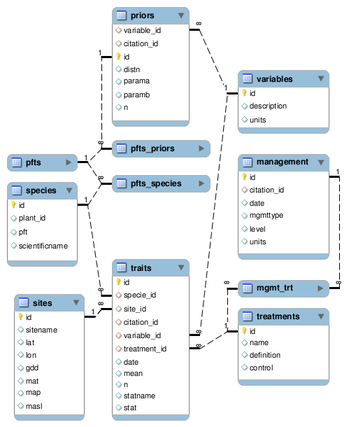
\includegraphics[width=3in]{summarymodel.png}
    \caption{Abbreviated schema for BETYdb \href{http://www.openwetware.org/images/d/d4/Summary_model20100713.jpg}{(Zoom)}.}
    \label{fig:summarymodel}
  \end{figure}
\end{centering}



\subsection{Data Access}\label{sec:download}
 Data is made available for analysis after it is submitted and reviewed by a database admistrator. 
 These data are suitable for basic scientific research and modeling. 
 All  reviewed data are made publicly available after publication to users of BETY-db who are conducting primary research.  
 Access to these raw data is provided to users based on affiliation and contribution of data.

 Data can be downloaded as a \verb+.csv=+ file, and data from previously published syntheses can be downloaded without login. 
 For example, to download all of the Switchgrass (\emph{Panicum virgatum} L.) yield data, 

\begin{enumerate}
\item Open the BETY homepage \href{ebi-forecast.igb.uiuc.edu/bety}{ebi-forecast.igb.uiuc.edu}
\item Select \href{http://ebi-forecast.igb.uiuc.edu/bety/maps/species_details}{\textbf{\texttt{Species database}}} under \textbf{Search}
\item Select \href{http://ebi-forecast.igb.uiuc.edu/bety/maps/yields?species=938}{\textbf{\texttt{Click Here}}} under Yields
\item to download all records as a comma-delimited (\verb+.csv+) file, scroll down and select the link \url{http://ebi-forecast.igb.uiuc.edu/bety/maps/yields?format=csv\&species=938}{\textbf{\texttt{CSV Format}} }
\end{enumerate}

\subsection{Web Interface}

 The web interface to BETYdb provides an interactive portal in which available data can be visualized, accessed, and entered (\autoref{fig:betyhome}).

\begin{centering}
  \begin{figure}[h]
    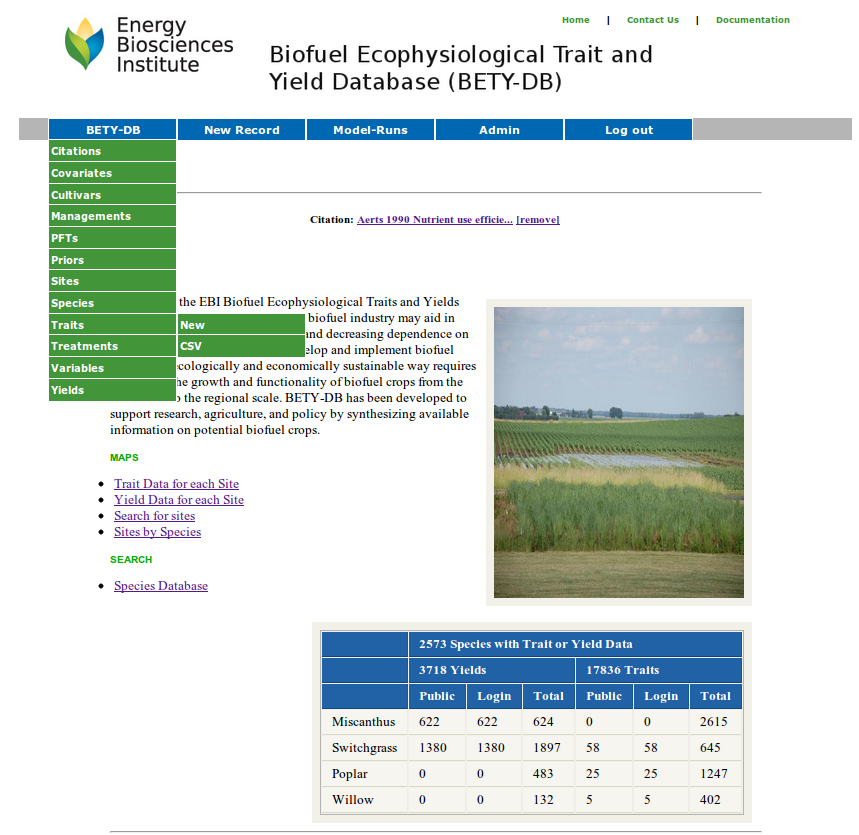
\includegraphics[width=5in]{betyhome.png}
    \caption{The BETYdb web interface home page.}
    \label{fig:betyhome}
  \end{figure}
\end{centering}

\subsection{Data Entry}

The \href{http://dl.dropbox.com/u/18092793/dbdocumentation_data_entry.pdf}{Data Entry Workflow} provides a complete description of the data entry process.
BETY's web interface has been developed to facilitate accurate and efficient data entry.
 This interface provides logical workflow to guide the user through comprehensively documenting data along with species, site information, and experimental methods.
 This workflow is outlined in the BETYdb Data Entry.
 Data entry requires a login with \verb+Create+ permissions, this can be obtained by contacting \href{mailto:dlebauer@illinois.edu}{David LeBauer} or \href{mailto:mdietze@illinois.edu}{Mike Dietze}.

\section{Tables}\label{sec:tables}

 The database is designed as a relationship database management system (RDBMS), following the normalization \autoref{fig:summarymodel}.
 Each table has a primary key field, \verb+id+, which is a unique identifier for each record in the table.
 In addition, each record has \verb+created_at+ and \verb+updated_at+ fields.
 The traits and yields tables each has a \verb+user_id+ field to record the user who originally entered the data.
 
 A complete list of tables is provided in \autoref{tab:tables}, and a comprehensive description of the contents of each table is provided below.  

\begin{table}[!htb]
\caption{Comprehensive list, overview, and brief description of tables in BETY}
\label{tab:tables}
\begin{tabular}{llHp{4in}}
\hline
Table &Name  & Use &  Description\\ \hline
\ref{tab:citations} & citations   &  & Citation information, links \\ 
\ref{tab:citations_sites}& citations\_sites        &  lookup & associates sites with citations\\ 
\ref{tab:citations_treatments}& citations\_treatments   &  lookup & associates citations with treatments \\ 
\ref{tab:covariates}& covariates   &  & covariates are required for some traits \\ 
\ref{tab:cultivars}& cultivars&  & cultivars associated with species \\
\ref{tab:error_logs}& error\_logs             &  & \\ 
\ref{tab:managements}& managements            &  & quantifies managements, including treatment levels; provides dates associated with treatments \\ 
\ref{tab:managements_treatments}& managements\_treatments & lookup & associates managements with specific treatments \\ 
\ref{tab:pfts}& pfts  &  & defines plant functional types (PFTs), users may choose existing pfts can be used, or user can enter pfts  \\ 
\ref{tab:pfts_priors}& pfts\_priors           & lookup & associates prior parameterizations with pfts used in modeling\\ 
\ref{tab:pfts_species}& pfts\_species           & lookup  & associates species with pfts used in modeling\\ 
\ref{tab:priors}& priors                 &  & PFT level summaries of available information for use in Bayesian meta-analysis\\ 
\ref{tab:sites}& sites                  &  & Site level information\\ 
\ref{tab:species}& species                &  & Based on USDA Plants database \\ 
\ref{tab:traits}& traits                 &  & Trait data table\\ 
\ref{tab:treatments}& treatments             &  & identifies experimental treatment name \\ 
%users table only for internal use 
%\ref{tab:users}& users}                  &  & controls data access levels, provides name and contact \\ 
\ref{tab:variables}& variables              &  & Description, including units, associated with variables used to define traits, trait covariates, and priors\\ 
\ref{tab:yields}& yields                 &  & Yield data table\\ \hline
\end{tabular} 
\end{table}

\subsection{Table and field naming conventions}
 Each table is given a name that describes the information that it contains.
 For example, the table containing trait data is called \verb+traits+, the table containing yield data is \verb+yields+, and so on.
 Each table also has a \emph{primary key}; the primary key is always \verb+id+, and the primary key of a specific table might be identified as \verb+yields.id+ . 
 One table can reference another table using a \emph{foreign key}; the foreign key is given a name using the singular form of the foreign table, and underscore, and id, e.g. \verb+traits_id+ or \verb+yields_id+.
 
 In some cases, two tables can have multiple references to one another, known as a 'many to many' or 'm:n' relationship. 
 For example, one citation may contain data from many sites; at the same time, data from a single site may be included in multiple citations.
 Such relationships use lookup tables.
 Lookup tables (e.g. Tables \ref{tab:citations_sites}, \ref{tab:citations_treatments}, \ref{tab:citations_sites}, \ref{tab:managements_treatments}, \ref{tab:pfts_priors}, \ref{tab:pfts_species}) combine the names of the two tables being related, in the case of this example, the table used to link \verb+citations+ and \verb+sites+ is named \verb+citations_sites+.
 These lookup tables have two foreign keys, e.g. \verb+citation_id+ and \verb+site_id+ but do not have a primary key 
 The foreign keys are identified by \texttt{FK: table.column} in the comment fields of the database tables where \texttt{table} is either a) for 1:many relationships the name of the master table in which \texttt{column} is the primary key or b) for many to many (m:n) relationships, to the auxillary table with \texttt{column} adjacent to another column with which the m:n relationship is simplified into 1:m and 1:n relationships.

\subsection{Data Tables}
 
 The two data tables, \textbf{traits} and \textbf{yields}, contain the primary data of interest; all of the other tables provide information associated with these data points.
 These two tables are structurally very similar as can be seen in Tables \ref{tab:traits} and \ref{tab:yields}.
 

\subsubsection{traits}

 The \textbf{traits} table contains trait data (\autoref{tab:traits}).
 Traits are measurable phenotypes that are influenced by a plants genotype and environment. 
 Most trait records presently in BETY describe tissue chemistry, photosynthetic parameters, and carbon allocation by plants.


\subsubsection{yields}
 
 The \textbf{yields} table includes aboveground biomass in units of Mg ha$^{-1}$  (\autoref{tab:yields}).
 Biomass harvested in the fall and winter generally represents what a farmer would harvest, whereas spring and summer harvests are generally from small samples used to monitor the progress of a crop over the course of the growing season.
 Managements associated with Yields can be used to determine the age of a crop, the fertilization history, harvest history, and other useful information.

\subsection{Auxillary Tables}

\subsubsection{sites}
 Each site is described in the \textbf{sites} table (\autoref{tab:sites}). 
 A site can have multiple studies and multiple treatments. Sites are identified and should be used as the unit of spatial replication; treatments are used identify independent units within a site, and these can be compared to other studies at the same site with shared management. 
 ''Studies'' are not identified explicitly but independent studies can be identified via shared management entries at the same site.  

\subsubsection{treatments}

The \textbf{treatments} table  provides a categorical identifier of a study's experimental treatments, if any (\autoref{tab:treatments}).

 Any specific information such as rate of fertilizer application should be recorded in the managements table (section.
 A treatment name is used as a categorical (rather than continuous) variable, and the name relates directly to the nomenclature used in the original citation.
 The treatment name does not have to indicate the level of treatment used in a particular treatment - if required for analysis, this information is recorded as a management.
 
 Each study includes a control treatment, when there is no experimental manipulation, the treatment is considered 'observational' and listed as control.
 In studies that compare plant traits or yields across different genotypes, site locations, or other factors that are built in to the database, each record is associated with a separate cultivar or site so these are not considered treatments.
 
 For ambiguous cases, the control treatment is assigned to the treatment that best approximates the background condition of the system in its non-experimental state, for this reason, a treatment that approximates conventional agronomic practice may be labeled 'control'.

\subsubsection{managements}

 The \textbf{managements} table provides information on management types, including planting time and methods, stand age, fertilization, irrigation, herbicides, pesticides, as well as harvest method, time and frequency. 

 The \textbf{managmenets} and \textbf{treatments} tables are linked through the \verb+managements_treatments+ lookup table (\ref{tab:managements_treatments}).

 Managements are distinct from treatments in that a management is used to describe the agronomic or experimental intervention that occurs at a specific time and may have a quantity whereas Treatment is a categorical identifier of an experimental group.
 Managements include actions that are done to a plant or ecosystem, for example the planting density or rate of fertilizer application.
 
 In other words, managements are the way a treatment becomes quantified. 
 Each treatment can be associated with multiple managements. 
 The combination of managements associated with a particular treatment will distinguish it from other treatments. 
 Each management may be associated with one or more treatments. 
 For example, in a fertilization experiment, planting, irrigation, and herbicide managements would be applied to all plots but the fertilization will be specific to a treatment.
For a multi-year experiment, there may be multiple entries for the same type of management, reflecting, for example, repeated applications of herbicide or fertilizer.



\subsubsection{covariates}

  The \textbf{covariates} table is used to record one or more covariates associated with each trait record  (\autoref{tab:covariates}). 
 Covariates generally indicate the environmental or experimental conditions under which a measurement was made.
 The definition of specific covariates can be found in the \textbf{variables} table (\autoref{tab:variables}).
 Covariates are required for many of the traits because without covariate information, the trait data will have limited value.
 
 The most frequently used covariates are the temperature at which some respiration rate or photosynthetic parameter was measured. 
 For example, photosynthesis measurements are often recorded along with irradiance, temperature, and relative humidity.

 Other covariates include the size or age of the plant or plant part being measured.
 For example, root respiration is usually measured on fine roots, and if the authors define fine root as <2mm, the covariate root\_minimum\_diameter has a value of $2$.


\subsubsection{pfts}

 The plant functional type (PFT) table, \textbf{pfts} is used to group plants for statistical modeling and analysis.
 Each record in \textbf{pfts} contains a PFT that is linked to a subset of species in the \textbf{species} table. 
 This relationship requires the lookup table \textbf{pfts\_species} (\autoref{tab:pfts_species}).
 Furtheromre, each PFT can be associated with a set of trait prior probability distributions in the \textbf{priors} table (\autoref{tab:priors}).
 This relationship requires the lookup table \textbf{pfts\_priors} (\autoref{tab:pfts_priors}).

 In many cases, it is appropriate to use a pre-defined default PFT (e.g. \verb+tempdecid+ is temperate deciduous trees)
 In other cases, a user can define a new pft to query a specific set of priors or subset of species.
 For example, there is a PFT for each of the functional types found at the EBI Farm prairie.
 Such project-specific PFTs can be defined as \verb+`projectname`.`pft`+ (i.e. \verb+ebifarm.c4grass+ instead of \verb+c4grass+).

%users table only for internal use 
%\subsubsection{users}

% The \textbf{users} table records basic user information and controls user access to data (\autoref{tab:users}).

% BETY has a two tiered access system, and each user is given an access level within each tier. 
% The first tier is controlled by the field \verb+page_access_level+ in the Users table.
% The  \verb+page_access_level+ field dictates which pages on the site a user can access. 
% The second tier is controlled by the \verb+access_level+ field.
% The \verb+access_level+ field dictates which trait or yield data are available to the user.
% This field is set in the User table, and each trait or yield record has an \verb+access_level+ field that controls data availability.

% The access system is heirarchical:  every level inherits permissions from the levels above it, and is then given additional privileges.
% For \verb+page_access_level+, we have four levels:

%\begin{description}
%\item[\textbf{1. Admin:}]  Can access everything.
%\item[\textbf{2. Managers:}]  Can access everything an admin can minus other Users information.
%\item[\textbf{3. Creators:}]  Can add (not edit at the moment) content, then view any content they have added.
%\item[\textbf{4. Viewers:}]  Can view content in any table, but data might be restricted by \verb+access_level+.
%\end{description}

%For \verb+data access_level+, we also have four levels. 
% By default all data entered is set to the \verb+access_level+ of the person who entered it.

%\begin{description}
%\item[\textbf{1. Dietze-Lab:}]  Can only be accessed by those with User \verb+access_level+ $= 1$, anyone with this level can access all data checked or not at all access levels.
%\item[\textbf{2. EBI Researchers:}]  Can be accessed by those who entered it or (User set at \verb+access_level+ $\le 2$ and the data has been 'checked')
%\item[\textbf{3. External Researchers:}]  Can be accessed by those who entered it or (User set at \verb+access_level+ $\le 3$ and the data has been 'checked')
%\item[\textbf{4. Public:}] - Can be accessed by who entered it or (User set at \verb+access_level+ $\le 4$ and the data has been 'checked')
%\end{description}


\subsubsection{variables} 
 The \textbf{variables} table includes definitions of different variables used in the traits, covariates, and priors tables  (\autoref{tab:variables}).
 Each variable has a \verb+name+ field, and is associated with a standardized value for \verb+units+.
 The \verb+description+ field provides additional information or context about the variable.

\subsection{Lookup Tables}

 Lookup tables are required when each record on one table can be related to many records on another table, and vice-versa; this is called a 'many to many' relationship.

\subsubsection{citations\_sites}
Because a single study can use multiple sites and multiple studies can use the same site, these relationships are tracked in the \textbf{citation\_sites} table (\autoref{tab:citations_sites}).

\subsubsection{citations\_treatments}
Because a single study can include multiple treatments and each treatment can be associated with multiple citations, these relationships are measured in \textbf{citations\_treatments} table (\autoref{tab:citations_treatments}).


\subsubsection{managements\_treatments}
 It is clear that one treatment can have many managements, e.g. tillage, planting, fertilization.
 It is also important to note that any managements applied to a control plot should, by definition, be associated with all of the treatments in an experiment; this is why the many-to-many lookup table \textbf{managements\_treatments} is required.

\subsubsection{pfts\_priors}
The \textbf{pfts\_priors} table allows a many to many relationship between the \textbf{pfts} and \textbf{priors} tables (\autoref{tab:pfts_priors}).
 This allows each pft to be associated with multiple priors and each prior to be associated with multiple pfts.

\subsubsection{pfts\_species}

The \textbf{pfts\_species} table allows a many to many relationship between the \textbf{pfts} and \textbf{species} tables (\autoref{tab:pfts_species}).

\section{Acknowlegments}
 BETY-db is a product of the Energy Biosciences Institute at the University of Illinois at Urbana-Champaign. 
 Funding for this research was provided by British Petroleum through a grant to the  Energy Biosciences institute.
 We gratefully acknowledge the great effort of other researchers who generously made their own data available for further study.
\newpage
\section{Appendix}

\subsection{Full Schema: Enhanced Entity-Relationship Model}%\label{sec:model}
\autoref{fig:model} provides a visualization of the complete schema, including interrelationships among tables, of the biofuel database. 

\begin{figure}[hbtp]
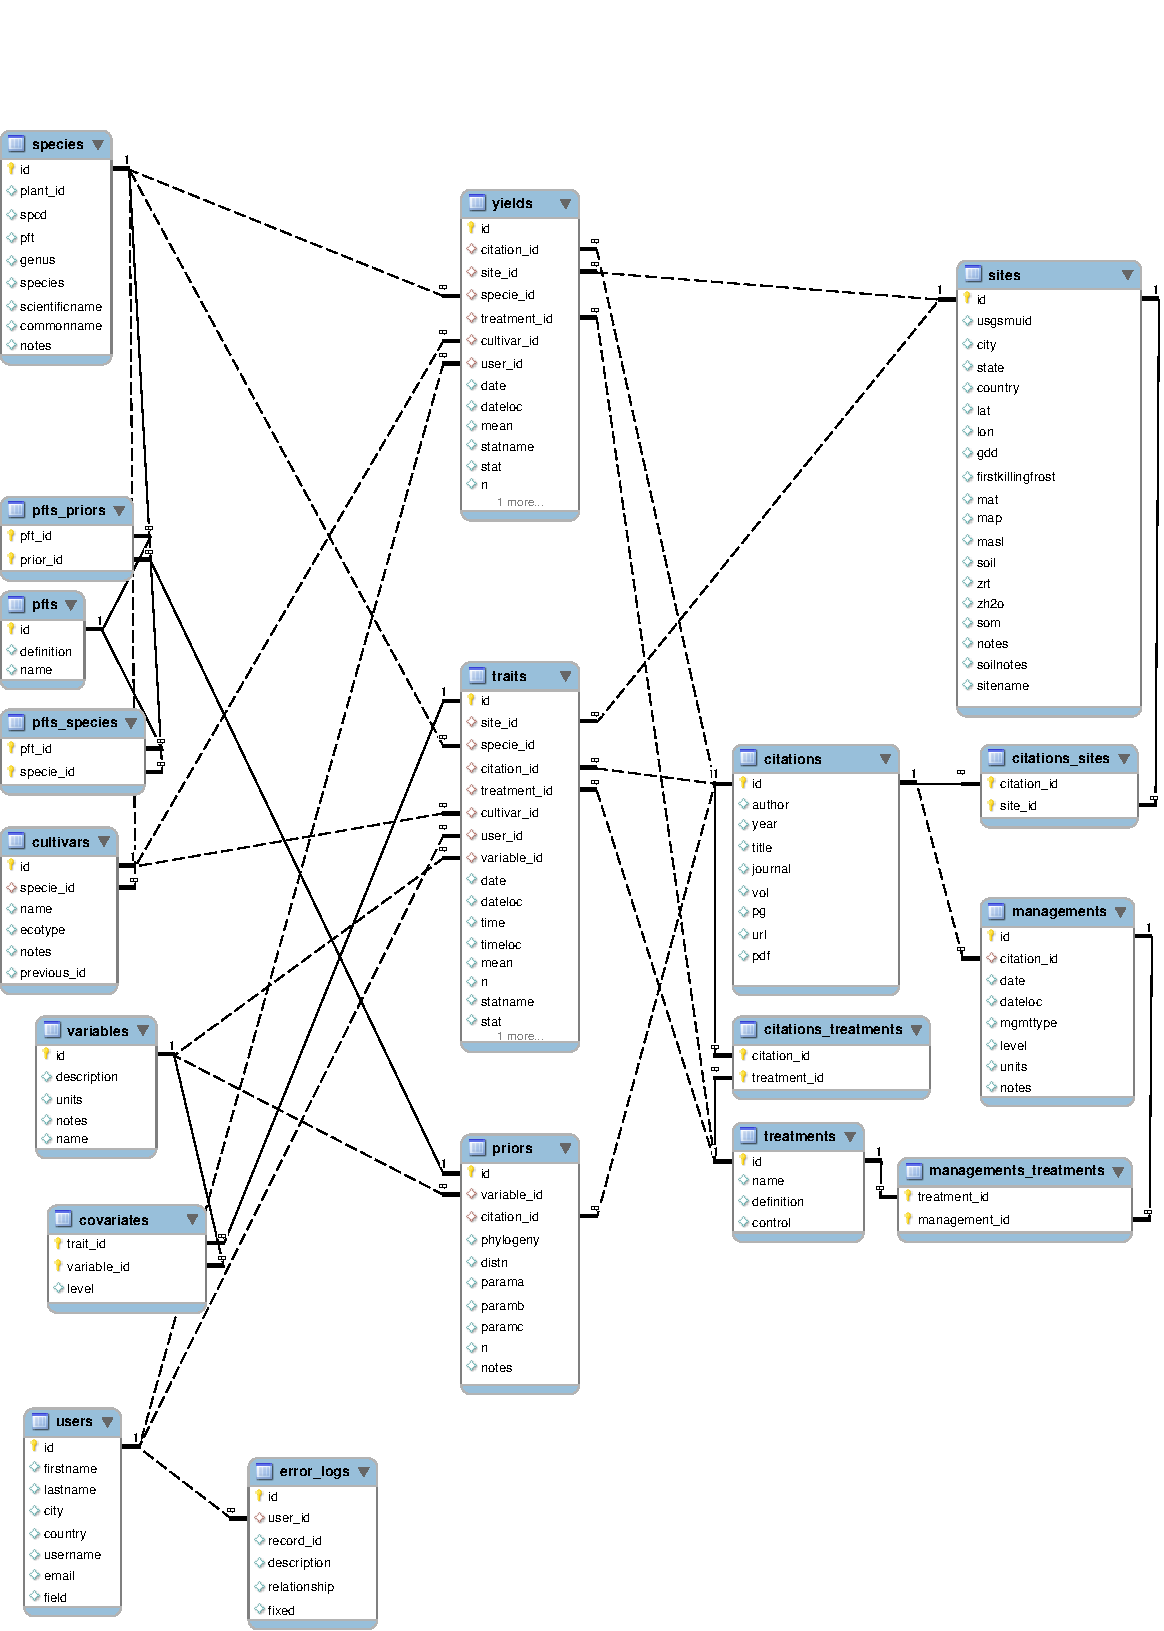
\includegraphics[width=\textwidth]{model.pdf}
\caption{Full Schema of BETYdb, showing all tables and relations in the database}
\label{fig:model}
\end{figure}

\subsection{Software}
 The BETY-db has beeen developed in MySQL using Ruby on Rails and is hosted on a RedHat Linux Server (ebi-forecast.igb.uiuc.edu). 
 BETY-db is a relational database designed in a generic way to facilitate easy implementation of additional traits and parameters. 

% \bibliographystyle{plainnat}
% \bibliography{bety_documentation_refs}


% \begin{table}[!htb]
%   \caption[Woody Species]{Species included in the novel woody crops trial.}
%   \label{tab:novelwoody}
%   \begin{tabular}{ll} \hline
%     Latin name  & Common name\\ \hline
%     \emph{Acer rubrum} & Red maple\\
%     \emph{Acer saccharinum} & Silver maple\\
%     \emph{Alnus incana tenuifolia} & Thinleaf alder\\
%     \emph{Betula nigra} & River birch\\
%     \emph{Castanea dentata} x \emph{C. mollissima} & Hybrid chestnut\\
%     \emph{Catalpa speciosa} & Northern catalpa\\
%     \emph{Celtis occidentalis} & Common hackberry\\
%     \emph{Cornus sanguinea} & Bloodtwig dogwood\\
%     \emph{Corylus americana} & American filbert\\
%     \emph{Cotinus obovatus} & American smoketree\\
%     \emph{Ilex decidua} & Possumhaw\\
%     \emph{Liquidambar styraciflua} & American Sweetgum\\
%     \emph{Liriodendron tulipifera} & Tuliptree\\
%     \emph{Maclura pomifera} & Osage orange\\
%     \emph{Platanus occidentalis} & Sycamore\\
%     \emph{Prunus serotina} & Black Cherry\\
%     \emph{Rhus copallinum} & Flameleaf sumac\\
%     \emph{Robinia pseudoacacia} & Black locust\\
%     \emph{Quercus coccinea} & Scarlet oak\\
%     \emph{Populus deltoides} & Eastern cottonwood\\
%     \emph{Pterocarya stenoptera} & Chinese wingnut\\
%     \emph{Salix} x Sherburne & Hybrid willow\\ \hline
%   \end{tabular}
% \end{table}


% \begin{table}[!htbp]
%   \caption[Prairie Species]{Prairie species included in the BETY database}
%   \label{tab:prairie}
%   \begin{tabular}{lll} \hline
%     PFT & scientificname & commonname\\ \hline
%     C3 Grass &  & \\
%     & \emph{Elymus repens} & quackgrass\\
%     & \emph{Koeleria macrantha} & prairie Junegrass\\
%     & \emph{Elymus canadensis} & Canada wildrye\\
%     & \emph{Poa pratensis} & \\
%     C4 Grass & & \\
%     & \emph{Panicum virgatum} & switchgrass\\
%     Nitrogen fixers &  & \\
%     & \emph{Astragalus canadensis} & \\
%     & \emph{Baptisia alba var. macrophylla} & largeleaf wild indigo\\
%     & \emph{Baptisia australis} & \\
%     & \emph{Baptisia bracteata var. laevicaulis} & \\
%     & \emph{Baptisia lanceolata} & \\
%     & \emph{Desmanthus illinoensis} & \\
%     & \emph{Lespedeza capitata} & roundhead lespedeza\\
%     Forb &  & \\
%     & \emph{Achillea millefolium} & \\
%     & \emph{Anemone cylindrica} & \\
%     & \emph{Coreopsis lanceolata} & \\
%     & \emph{Coreopsis tripteris} & tall tickseed\\
%     & \emph{Echinacea angustifolia} & \\
%     & \emph{Echinacea pallida} & \\
%     & \emph{Echinacea purpurea} & \\
%     & \emph{Echinacea tennesseensis} & \\
%     & \emph{Helenium linifolium} & \\
%     & \emph{Helianthus grosseserratus} & sawtooth sunflower\\
%     & \emph{Helianthus maximiliani} & \\
%     & \emph{Heliopsis helianthoides} & smooth oxeye\\
%     & \emph{Hypericum perforatum} & \\
%     & \emph{Liatris pycnostachya} & \\
%     & \emph{Monarda fistulosa} & \\
%     & \emph{Oligoneuron ohioense} & \\
%     & \emph{Parthenium integrifolium} & \\
%     & \emph{Penstemon digitalis} & \\
%     & \emph{Ratibida pinnata} & pinnate prairie coneflower\\
%     & \emph{Rudbeckia subtomentosa} & sweet coneflower\\
%     & \emph{Silphium integrifolium} & wholeleaf rosinweed\\
%     & \emph{Silphium laciniatum} & \\
%     & \emph{Silphium perfoliatum} & \\
%     & \emph{Silphium trifoliatum} & \\
%     & \emph{Solidago altissima} & Canada goldenrod\\
%     & \emph{Solidago canadensis} & \\
%     & \emph{Solidago rugosa} & \\
%     & \emph{Solidago speciosa} & \\
%     & \emph{Veronicastrum virginicum} & \\ \hline
%   \end{tabular}
% \end{table}
% \clearpage


% \begin{table}[!htb]
%   \begin{tabular}{lll} \hline
%     Trait & observations & Citation \\ \hline 
%     SLA &  & \citep{wright2004wwl}\\ %citation_id = 160
%     leaf \%N & & \citep{reich2004gpp}\\ %select distinct variable_id from traits where citation_id = 30; 
%     leaf \%P & & \citep{reich2004gpp}\\ %select distinct variable_id from traits where citation_id = 30; 
%     Vc$_\text{max}$ & & \citep{wullschleger1993blc} \\ 
%     J$_\text{max}$ & & \citep{wullschleger1993blc} \\ 
%     \hline
%   \end{tabular}
%   \caption[External Data available throug BETYdb]{Data from external summaries included in BETYdb}
%   \label{tab:externaldata}
% \end{table}


 \begin{longtable}[!htb]{lcccp{2in}H} 
 \caption{citations table} \label{tab:citations} \\
 \toprule  \multicolumn{1}{c}{\textbf{Field}} & \multicolumn{1}{c}{\textbf{Type}} & \multicolumn{1}{c}{\textbf{Null}} & \multicolumn{1}{c}{\textbf{Default}} & \multicolumn{1}{c}{\textbf{Comments}} & \multicolumn{1}{c}{\textbf{}} \\  
\midrule \endfirsthead
 \caption{citations table (continued)} \\ 
 \toprule  \multicolumn{1}{c}{\textbf{Field}} & \multicolumn{1}{c}{\textbf{Type}} & \multicolumn{1}{c}{\textbf{Null}} & \multicolumn{1}{c}{\textbf{Default}} & \multicolumn{1}{c}{\textbf{Comments}} & \multicolumn{1}{c}{\textbf{}} \\   \midrule  \endhead  \endfoot       
\textbf{\textit{id}} & int(11) & No &  &  &  \\  
Field & Type & Null & Default & Comments & \\ 
id & int(11) & No &  &  & \\ 
author & varchar(255) & Yes & NULL & last name of first author & \\ 
year & int(11) & Yes & NULL & year of publication & \\ 
title & varchar(255) & Yes & NULL & article title & \\ 
journal & varchar(255) & Yes & NULL & Journal name & \\ 
vol & int(11) & Yes & NULL &  & \\ 
pg & varchar(255) & Yes & NULL & page range of article & \\ 
url & varchar(512) & Yes & NULL & link to article url & \\ 
pdf & varchar(255) & Yes & NULL & link to pdf version of article & \\ 
created\_at & datetime & Yes & NULL &  & \\ 
updated\_at & datetime & Yes & NULL &  & \\ 
doi & varchar(255) & Yes & NULL & Digital Object Identifier & \\ 
\bottomrule  \end{longtable}

%
% Structure: citations_sites
%
 \begin{longtable}[!htb]{lcccp{2in}H}
 \caption{citations\_sites table} \label{tab:citations_sites} \\
 \toprule  \multicolumn{1}{c}{\textbf{Field}} & \multicolumn{1}{c}{\textbf{Type}} & \multicolumn{1}{c}{\textbf{Null}} & \multicolumn{1}{c}{\textbf{Default}} & \multicolumn{1}{c}{\textbf{Comments}} & \multicolumn{1}{c}{\textbf{}} \\  
\midrule \endfirsthead
 \caption{citations\_sites table (continued)} \\ 
 \toprule  \multicolumn{1}{c}{\textbf{Field}} & \multicolumn{1}{c}{\textbf{Type}} & \multicolumn{1}{c}{\textbf{Null}} & \multicolumn{1}{c}{\textbf{Default}} & \multicolumn{1}{c}{\textbf{Comments}} & \multicolumn{1}{c}{\textbf{}} \\   \midrule  \endhead  \endfoot
citation\_id & int(11) & Yes & NULL &  & \\ 
site\_id & int(11) & Yes & NULL &  & \\ 
created\_at & datetime & Yes & NULL &  & \\ 
updated\_at & datetime & Yes & NULL &  & \\ 
\bottomrule  \end{longtable}

%
% Structure: citations_treatments
%
 \begin{longtable}[!htb]{lcccp{2in}H} 
 \caption{citations\_treatments table} \label{tab:citations_treatments} \\
 \toprule  \multicolumn{1}{c}{\textbf{Field}} & \multicolumn{1}{c}{\textbf{Type}} & \multicolumn{1}{c}{\textbf{Null}} & \multicolumn{1}{c}{\textbf{Default}} & \multicolumn{1}{c}{\textbf{Comments}} & \multicolumn{1}{c}{\textbf{}} \\  
\midrule \endfirsthead
 \caption{citations\_treatments table (continued)} \\ 
 \toprule  \multicolumn{1}{c}{\textbf{Field}} & \multicolumn{1}{c}{\textbf{Type}} & \multicolumn{1}{c}{\textbf{Null}} & \multicolumn{1}{c}{\textbf{Default}} & \multicolumn{1}{c}{\textbf{Comments}} & \multicolumn{1}{c}{\textbf{}} \\   \midrule  \endhead  \endfoot
\textbf{citation\_id} & int(11) & Yes & NULL &  &  \\  
\textbf{treatment\_id} & int(11) & Yes & NULL &  &  \\  
created\_at & datetime & Yes & NULL &  &  \\  
updated\_at & datetime & Yes & NULL &  &  \\  
\bottomrule  \end{longtable}

%
%
%
% Structure: covariates
%
 \begin{longtable}[!htb]{lcccp{2in}H} 
 \caption{covariates table} \label{tab:covariates} \\
 \toprule  \multicolumn{1}{c}{\textbf{Field}} & \multicolumn{1}{c}{\textbf{Type}} & \multicolumn{1}{c}{\textbf{Null}} & \multicolumn{1}{c}{\textbf{Default}} & \multicolumn{1}{c}{\textbf{Comments}} & \multicolumn{1}{c}{\textbf{}} \\  
\midrule \endfirsthead
 \caption{covariates table (continued)} \\ 
 \toprule  \multicolumn{1}{c}{\textbf{Field}} & \multicolumn{1}{c}{\textbf{Type}} & \multicolumn{1}{c}{\textbf{Null}} & \multicolumn{1}{c}{\textbf{Default}} & \multicolumn{1}{c}{\textbf{Comments}} & \multicolumn{1}{c}{\textbf{}} \\   \midrule  \endhead  \endfoot
id & int(11) & No &  &  & \\ 
trait\_id & int(11) & Yes & NULL &  & \\ 
variable\_id & int(11) & Yes & NULL &  & \\ 
level & decimal(16,4) & Yes & NULL & Value of covariate, units are determined in variables table by the variable\_id foreign key. & \\ 
created\_at & datetime & Yes & NULL &  & \\ 
updated\_at & datetime & Yes & NULL &  & \\ 
\bottomrule  \end{longtable}

%
% Structure: cultivars
%
 \begin{longtable}[!htb]{lcccp{2in}H} 
 \caption{cultivars table} \label{tab:cultivars} \\
 \toprule  \multicolumn{1}{c}{\textbf{Field}} & \multicolumn{1}{c}{\textbf{Type}} & \multicolumn{1}{c}{\textbf{Null}} & \multicolumn{1}{c}{\textbf{Default}} & \multicolumn{1}{c}{\textbf{Comments}} & \multicolumn{1}{c}{\textbf{}} \\  
\midrule \endfirsthead
 \caption{cultivars table (continued)} \\ 
 \toprule  \multicolumn{1}{c}{\textbf{Field}} & \multicolumn{1}{c}{\textbf{Type}} & \multicolumn{1}{c}{\textbf{Null}} & \multicolumn{1}{c}{\textbf{Default}} & \multicolumn{1}{c}{\textbf{Comments}} & \multicolumn{1}{c}{\textbf{}} \\   \midrule  \endhead  \endfoot
id & int(11) & No &  &  & \\ 
specie\_id & int(11) & Yes & NULL &  & \\ 
name & varchar(255) & Yes & NULL & Cultivar name given by breeder or reported in citation. & \\ 
ecotype & varchar(255) & Yes & NULL & Does not apply for all species, used in the case of switchgrass to differentiate lowland and upland genotypes. & \\ 
notes & text & Yes & NULL &  & \\ 
created\_at & datetime & Yes & NULL &  & \\ 
updated\_at & datetime & Yes & NULL &  & \\ 
previous\_id & varchar(255) & Yes & NULL &  & \\ 
\bottomrule  \end{longtable}

%
% Structure: error_logs
%
 \begin{longtable}[!htb]{lcccp{2in}H} 
 \caption{error\_logs table} \label{tab:error_logs} \\
 \toprule  \multicolumn{1}{c}{\textbf{Field}} & \multicolumn{1}{c}{\textbf{Type}} & \multicolumn{1}{c}{\textbf{Null}} & \multicolumn{1}{c}{\textbf{Default}} & \multicolumn{1}{c}{\textbf{Comments}} & \multicolumn{1}{c}{\textbf{}} \\  
\midrule \endfirsthead
 \caption{error\_logs table (continued)} \\ 
 \toprule  \multicolumn{1}{c}{\textbf{Field}} & \multicolumn{1}{c}{\textbf{Type}} & \multicolumn{1}{c}{\textbf{Null}} & \multicolumn{1}{c}{\textbf{Default}} & \multicolumn{1}{c}{\textbf{Comments}} & \multicolumn{1}{c}{\textbf{}} \\   \midrule  \endhead  \endfoot
id & int(11) & No &  &  & \\ 
record\_id & int(11) & Yes & NULL &  & \\ 
description & varchar(255) & Yes & NULL & Description of error that needs to be addressed. & \\ 
relationship & varchar(255) & Yes & NULL &  & \\ 
user\_id & int(11) & Yes & NULL & Identifies user responsible for handling error. & \\ 
fixed & int(11) & Yes & \multicolumn{1}{r}{0} & Set to 0 when error is reported, 1 after error has been checked and fixed. & \\ 
created\_at & datetime & Yes & NULL &  & \\ 
updated\_at & datetime & Yes & NULL &  & \\ 
\bottomrule  \end{longtable}

%
% Structure: managements
%
 \begin{longtable}[!htb]{lcccp{2in}H} 
 \caption{managements table} \label{tab:managements} \\
 \toprule  \multicolumn{1}{c}{\textbf{Field}} & \multicolumn{1}{c}{\textbf{Type}} & \multicolumn{1}{c}{\textbf{Null}} & \multicolumn{1}{c}{\textbf{Default}} & \multicolumn{1}{c}{\textbf{Comments}} & \multicolumn{1}{c}{\textbf{}} \\  
\midrule \endfirsthead
 \caption{managements table (continued)} \\ 
 \toprule  \multicolumn{1}{c}{\textbf{Field}} & \multicolumn{1}{c}{\textbf{Type}} & \multicolumn{1}{c}{\textbf{Null}} & \multicolumn{1}{c}{\textbf{Default}} & \multicolumn{1}{c}{\textbf{Comments}} & \multicolumn{1}{c}{\textbf{}} \\   \midrule  \endhead  \endfoot

id & int(11) & No &  &  & \\ 
citation\_id & int(11) & Yes & NULL &  & \\ 
date & date & Yes & NULL & Date on which management was conducted. & \\ 
dateloc & decimal(4,2) & Yes & NULL & Level of confidence in value given as date. See documentation for details. & \\ 
mgmttype & varchar(255) & Yes & NULL & Type of management & \\ 
level & decimal(16,4) & Yes & NULL & Amount applied, not always required. & \\ 
units & varchar(255) & Yes & NULL & units, standardized for each management type. & \\ 
notes & text & Yes & NULL &  & \\ 
created\_at & datetime & Yes & NULL &  & \\ 
updated\_at & datetime & Yes & NULL &  & \\ 

\bottomrule  \end{longtable}

%
% Structure: managements_treatments
%
 \begin{longtable}[!htb]{lcccp{2in}H} 
 \caption{managements\_treatments table} \label{tab:managements_treatments} \\
 \toprule  \multicolumn{1}{c}{\textbf{Field}} & \multicolumn{1}{c}{\textbf{Type}} & \multicolumn{1}{c}{\textbf{Null}} & \multicolumn{1}{c}{\textbf{Default}} & \multicolumn{1}{c}{\textbf{Comments}} & \multicolumn{1}{c}{\textbf{}} \\  
\midrule \endfirsthead
 \caption{managements\_treatments table (continued)} \\ 
 \toprule  \multicolumn{1}{c}{\textbf{Field}} & \multicolumn{1}{c}{\textbf{Type}} & \multicolumn{1}{c}{\textbf{Null}} & \multicolumn{1}{c}{\textbf{Default}} & \multicolumn{1}{c}{\textbf{Comments}} & \multicolumn{1}{c}{\textbf{}} \\   \midrule  \endhead  \endfoot
\textbf{treatment\_id} & int(11) & Yes & NULL &  &  \\  
\textbf{management\_id} & int(11) & Yes & NULL &  &  \\  
created\_at & datetime & Yes & NULL &  &  \\  
updated\_at & datetime & Yes & NULL &  &  \\  
\bottomrule  \end{longtable}

%
% Structure: pfts
%
 \begin{longtable}[!htb]{lcccp{2in}H} 
 \caption{pfts table} \label{tab:pfts} \\
 \toprule  \multicolumn{1}{c}{\textbf{Field}} & \multicolumn{1}{c}{\textbf{Type}} & \multicolumn{1}{c}{\textbf{Null}} & \multicolumn{1}{c}{\textbf{Default}} & \multicolumn{1}{c}{\textbf{Comments}} & \multicolumn{1}{c}{\textbf{}} \\  
\midrule \endfirsthead
 \caption{pfts table (continued)} \\ 
 \toprule  \multicolumn{1}{c}{\textbf{Field}} & \multicolumn{1}{c}{\textbf{Type}} & \multicolumn{1}{c}{\textbf{Null}} & \multicolumn{1}{c}{\textbf{Default}} & \multicolumn{1}{c}{\textbf{Comments}} & \multicolumn{1}{c}{\textbf{}} \\   \midrule  \endhead  \endfoot

id & int(11) & No &  &  & \\ 
definition & text & Yes & NULL & Defines the creator and context under which the pft will be used. & \\ 
created\_at & datetime & Yes & NULL &  & \\ 
updated\_at & datetime & Yes & NULL &  & \\ 
name & varchar(255) & Yes & NULL & unique identifier used by PEcAn. & \\ 
\bottomrule  \end{longtable}
% Structure: pfts_priors
%
 \begin{longtable}[!htb]{lcccp{2in}H} 
 \caption{pfts\_priors table} \label{tab:pfts_priors} \\
 \toprule  \multicolumn{1}{c}{\textbf{Field}} & \multicolumn{1}{c}{\textbf{Type}} & \multicolumn{1}{c}{\textbf{Null}} & \multicolumn{1}{c}{\textbf{Default}} & \multicolumn{1}{c}{\textbf{Comments}} & \multicolumn{1}{c}{\textbf{}} \\  
\midrule \endfirsthead
 \caption{pfts\_priors table (continued)} \\ 
 \toprule  \multicolumn{1}{c}{\textbf{Field}} & \multicolumn{1}{c}{\textbf{Type}} & \multicolumn{1}{c}{\textbf{Null}} & \multicolumn{1}{c}{\textbf{Default}} & \multicolumn{1}{c}{\textbf{Comments}} & \multicolumn{1}{c}{\textbf{}} \\   \midrule  \endhead  \endfoot
pft\_id & int(11) & Yes & NULL &  & \\ 
prior\_id & int(11) & Yes & NULL &  & \\ 
created\_at & datetime & Yes & NULL &  & \\ 
updated\_at & datetime & Yes & NULL &  & \\ 
\bottomrule  \end{longtable}

%
%
%
% Structure: pfts_species
%
 \begin{longtable}[!htb]{lcccp{2in}H} 
 \caption{pfts\_species table} \label{tab:pfts_species} \\
 \toprule  \multicolumn{1}{c}{\textbf{Field}} & \multicolumn{1}{c}{\textbf{Type}} & \multicolumn{1}{c}{\textbf{Null}} & \multicolumn{1}{c}{\textbf{Default}} & \multicolumn{1}{c}{\textbf{Comments}} & \multicolumn{1}{c}{\textbf{}} \\  
\midrule \endfirsthead
 \caption{pfts\_species table (continued)} \\ 
 \toprule  \multicolumn{1}{c}{\textbf{Field}} & \multicolumn{1}{c}{\textbf{Type}} & \multicolumn{1}{c}{\textbf{Null}} & \multicolumn{1}{c}{\textbf{Default}} & \multicolumn{1}{c}{\textbf{Comments}} & \multicolumn{1}{c}{\textbf{}} \\   \midrule  \endhead  \endfoot
pft\_id & int(11) & Yes & NULL &  & \\ 
specie\_id & int(11) & Yes & NULL &  & \\ 
created\_at & datetime & Yes & NULL &  & \\ 
updated\_at & datetime & Yes & NULL &  & \\ 
\bottomrule  \end{longtable}

%
% Structure: priors
%
 \begin{longtable}[!htb]{lcccp{2in}H} 
 \caption{priors table} \label{tab:priors} \\
 \toprule  \multicolumn{1}{c}{\textbf{Field}} & \multicolumn{1}{c}{\textbf{Type}} & \multicolumn{1}{c}{\textbf{Null}} & \multicolumn{1}{c}{\textbf{Default}} & \multicolumn{1}{c}{\textbf{Comments}} & \multicolumn{1}{c}{\textbf{}} \\  
\midrule \endfirsthead
 \caption{priors table (continued)} \\ 
 \toprule  \multicolumn{1}{c}{\textbf{Field}} & \multicolumn{1}{c}{\textbf{Type}} & \multicolumn{1}{c}{\textbf{Null}} & \multicolumn{1}{c}{\textbf{Default}} & \multicolumn{1}{c}{\textbf{Comments}} & \multicolumn{1}{c}{\textbf{}} \\   \midrule  \endhead  \endfoot
id & int(11) & No &  &  & \\ 
citation\_id & int(11) & Yes & NULL &  & \\ 
variable\_id & varchar(255) & Yes & NULL & Links to variable for which prior is used. & \\ 
phylogeny & varchar(255) & Yes & NULL & Used to note the group of plants for which the prior was specified, often the group of plants represented by the data used to specify the prior. & \\ 
distn & varchar(255) & Yes & NULL & Name of the probability distribution, using R naming convention (e.g. 'beta','f', 'gamma', 'lnorm', 'norm', 'pois', 't', 'unif', 'weibull'. & \\ 
parama & decimal(16,4) & Yes & NULL & First parameter for distribution, as specified by R. & \\ 
paramb & decimal(16,4) & Yes & NULL & Second parameter for distribution, as specified by R. & \\ 
paramc & decimal(16,4) & Yes & NULL & A third parameter, if required. & \\ 
n & int(11) & Yes & NULL & number of observations used to specify prior. & \\ 
notes & text & Yes & NULL &  & \\ 
created\_at & datetime & Yes & NULL &  & \\ 
updated\_at & datetime & Yes & NULL &  & \\ 
\bottomrule  \end{longtable}
%
% Structure: sites
%
 \begin{longtable}[!htb]{lcccp{2in}H} 
 \caption{sites table} \label{tab:sites} \\
 \toprule  \multicolumn{1}{c}{\textbf{Field}} & \multicolumn{1}{c}{\textbf{Type}} & \multicolumn{1}{c}{\textbf{Null}} & \multicolumn{1}{c}{\textbf{Default}} & \multicolumn{1}{c}{\textbf{Comments}} & \multicolumn{1}{c}{\textbf{}} \\  
\midrule \endfirsthead
 \caption{sites table (continued)} \\ 
 \toprule  \multicolumn{1}{c}{\textbf{Field}} & \multicolumn{1}{c}{\textbf{Type}} & \multicolumn{1}{c}{\textbf{Null}} & \multicolumn{1}{c}{\textbf{Default}} & \multicolumn{1}{c}{\textbf{Comments}} & \multicolumn{1}{c}{\textbf{}} \\   \midrule  \endhead  \endfoot

id & int(11) & No &  &  & \\ 
usgsmuid & varchar(255) & Yes & NULL &  & \\ 
city & varchar(255) & Yes & NULL & Nearest city to site. & \\ 
state & varchar(255) & Yes & NULL & If in the United States, state in which study is conducted. & \\ 
country & varchar(255) & Yes & NULL &  & \\ 
lat & decimal(9,6) & Yes & NULL & Latitude, in decimal degrees & \\ 
lon & decimal(9,6) & Yes & NULL & Longitude, in decimal degrees. & \\ 
gdd & int(11) & Yes & NULL & Depreciated & \\ 
firstkillingfrost & date & Yes & NULL & Depreciated & \\ 
mat & int(11) & Yes & NULL & Mean Annual Temperature (C) & \\ 
map & int(11) & Yes & NULL & Mean Annual Precipitation (mm) & \\ 
masl & int(11) & Yes & NULL & Elevation (m above sea level) & \\ 
soil & varchar(255) & Yes & NULL & Soil type,  'sand', 'loamy sand', 'sandy loam', 'silt loam', 'loam', 'sandy clay loam', 'silty clay loam', 'clay loam', 'sandy clay', 'silty clay', 'clay', 'peat'. & \\ 
zrt & decimal(4,2) & Yes & NULL & Depreciated & \\ 
zh2o & decimal(4,1) & Yes & NULL & Depreciated & \\ 
som & decimal(4,2) & Yes & NULL & Depreciated & \\ 
notes & text & Yes & NULL &  & \\ 
soilnotes & text & Yes & NULL &  & \\ 
created\_at & datetime & Yes & NULL &  & \\ 
updated\_at & datetime & Yes & NULL &  & \\ 
sitename & varchar(255) & Yes & NULL &  & \\ 
greenhouse & tinyint(1) & Yes & NULL & Boolean: indicates if study was conducted in a field (0) or greenhouse, pot, or growth chamber (1) & \\ 
\bottomrule  \end{longtable}


%
% Structure: species
%
 \begin{longtable}[!htb]{lcccp{2in}H} 
 \caption{species table} \label{tab:species} \\
 \toprule  \multicolumn{1}{c}{\textbf{Field}} & \multicolumn{1}{c}{\textbf{Type}} & \multicolumn{1}{c}{\textbf{Null}} & \multicolumn{1}{c}{\textbf{Default}} & \multicolumn{1}{c}{\textbf{Comments}} & \multicolumn{1}{c}{\textbf{}} \\  
\midrule \endfirsthead
 \caption{species table (continued)} \\ 
 \toprule  \multicolumn{1}{c}{\textbf{Field}} & \multicolumn{1}{c}{\textbf{Type}} & \multicolumn{1}{c}{\textbf{Null}} & \multicolumn{1}{c}{\textbf{Default}} & \multicolumn{1}{c}{\textbf{Comments}} & \multicolumn{1}{c}{\textbf{}} \\   \midrule  \endhead  \endfoot
id & int(11) & No &  &  & \\ 
plant\_id & int(11) & Yes & NULL &  & \\ 
spcd & int(11) & Yes & NULL &  & \\ 
pft & int(11) & Yes & NULL & Depreciated: moved to pfts\_species table & \\ 
genus & varchar(255) & Yes & NULL &  & \\ 
species & varchar(255) & Yes & NULL &  & \\ 
scientificname & varchar(255) & Yes & NULL &  & \\ 
commonname & varchar(255) & Yes & NULL &  & \\ 
notes & varchar(255) & Yes & NULL &  & \\ 
created\_at & datetime & Yes & NULL &  & \\ 
updated\_at & datetime & Yes & NULL &  & \\ 
... &  &  & & other columns imported from \href{http://plants.usda.gov}{USDA Plants database}  & \\ 
\bottomrule  \end{longtable}

%
% Structure: traits
%
 \begin{longtable}[!htb]{lcccp{2in}H} 
 \caption{traits table} \label{tab:traits} \\
 \toprule  \multicolumn{1}{c}{\textbf{Field}} & \multicolumn{1}{c}{\textbf{Type}} & \multicolumn{1}{c}{\textbf{Null}} & \multicolumn{1}{c}{\textbf{Default}} & \multicolumn{1}{c}{\textbf{Comments}} & \multicolumn{1}{c}{\textbf{}} \\  
\midrule \endfirsthead
 \caption{traits table (continued)} \\ 
 \toprule  \multicolumn{1}{c}{\textbf{Field}} & \multicolumn{1}{c}{\textbf{Type}} & \multicolumn{1}{c}{\textbf{Null}} & \multicolumn{1}{c}{\textbf{Default}} & \multicolumn{1}{c}{\textbf{Comments}} & \multicolumn{1}{c}{\textbf{}} \\   \midrule  \endhead  \endfoot
id & int(11) & No &  &  & \\ 
site\_id & int(11) & Yes & NULL & Site at which measurement was taken. & \\ 
specie\_id & int(11) & Yes & NULL & Species on which measurement was taken. & \\ 
citation\_id & int(11) & Yes & NULL & Citation in which data was originally reported. & \\ 
cultivar\_id & int(11) & Yes & NULL & Cultivar information, if any. & \\ 
treatment\_id & int(11) & Yes & NULL & Experimental treatment identification. Required, can indicate observational study. & \\ 
date & datetime & Yes & NULL & Date on which measurement was made. & \\ 
dateloc & decimal(4,2) & Yes & NULL & Level of confidence in date. See documentation. & \\ 
time & time & Yes & NULL & Time at which measurement was taken. Sometimes necessary, e.g. for photosynthesis measurements. & \\ 
timeloc & decimal(4,2) & Yes & NULL & Level of confidence in time. & \\ 
mean & decimal(16,4) & Yes & NULL & Mean value of trait. & \\ 
n & int(11) & Yes & NULL & Number of experimental replicates used to estimate mean and statistical summary. & \\ 
statname & varchar(255) & Yes & NULL & Name of reported statistic. & \\ 
stat & decimal(16,4) & Yes & NULL & Value of reported statistic. & \\ 
notes & text & Yes & NULL &  & \\ 
created\_at & datetime & Yes & NULL &  & \\ 
updated\_at & datetime & Yes & NULL &  & \\ 
variable\_id & int(11) & Yes & NULL & Links to information in variables table that describes trait being measured.  & \\ 
user\_id & int(11) & Yes & NULL & ID of user who entered data. & \\ 
checked & tinyint(1) & Yes & \multicolumn{1}{r}{0} & Boolean, indicates if data have been checked after original entry. & \\ 
access\_level & int(11) & Yes & NULL & Level of access required to view data. & \\ 
\bottomrule  \end{longtable}


%
% Structure: treatments
%
 \begin{longtable}[!htb]{lcccp{2in}H} 
 \caption{treatments table} \label{tab:treatments} \\
 \toprule  \multicolumn{1}{c}{\textbf{Field}} & \multicolumn{1}{c}{\textbf{Type}} & \multicolumn{1}{c}{\textbf{Null}} & \multicolumn{1}{c}{\textbf{Default}} & \multicolumn{1}{c}{\textbf{Comments}} & \multicolumn{1}{c}{\textbf{}} \\  
\midrule \endfirsthead
 \caption{treatments table (continued)} \\ 
 \toprule  \multicolumn{1}{c}{\textbf{Field}} & \multicolumn{1}{c}{\textbf{Type}} & \multicolumn{1}{c}{\textbf{Null}} & \multicolumn{1}{c}{\textbf{Default}} & \multicolumn{1}{c}{\textbf{Comments}} & \multicolumn{1}{c}{\textbf{}} \\   \midrule  \endhead  \endfoot
id & int(11) & No &  &  & \\ 
name & varchar(255) & Yes & NULL & Name of treatment, should be easy to associate with treatment name in original study. & \\ 
definition & varchar(255) & Yes & NULL & Description of treatment, e.g. levels of fertilizer applied, etc. This information may be redundant with 'levels' information recorded in Managements table. & \\ 
created\_at & datetime & Yes & NULL &  & \\ 
updated\_at & datetime & Yes & NULL &  & \\ 
control & tinyint(1) & Yes & NULL & Boolean, indicates if treatment is a control or observational (1) or experimental treatment (0). & \\ 
\bottomrule  \end{longtable}


% Users table removed from public documentation
% Structure: users
%
%  \begin{longtable}[!htb]{lcccp{2in}H} 
%  \caption{users table} \label{tab:users} \\
%  \toprule  \multicolumn{1}{c}{\textbf{Field}} & \multicolumn{1}{c}{\textbf{Type}} & \multicolumn{1}{c}{\textbf{Null}} & \multicolumn{1}{c}{\textbf{Default}} & \multicolumn{1}{c}{\textbf{Comments}} & \multicolumn{1}{c}{\textbf{}} \\  
% \midrule \endfirsthead
%  \caption{users table (continued)} \\ 
%  \toprule  \multicolumn{1}{c}{\textbf{Field}} & \multicolumn{1}{c}{\textbf{Type}} & \multicolumn{1}{c}{\textbf{Null}} & \multicolumn{1}{c}{\textbf{Default}} & \multicolumn{1}{c}{\textbf{Comments}} & \multicolumn{1}{c}{\textbf{}} \\   \midrule  \endhead  \endfoot

% id & int(11) & No &  &  & \\ 
% login & varchar(40) & Yes & NULL & login id & \\ 
% name & varchar(100) & Yes &  & User name & \\ 
% email & varchar(100) & Yes & NULL & email address & \\ 
% city & varchar(255) & Yes & NULL &  & \\ 
% country & varchar(255) & Yes & NULL &  & \\ 
% field & varchar(255) & Yes & NULL & field of work (e.g. academic, industry, agriculture) & \\ 
% crypted\_password & varchar(40) & Yes & NULL &  & \\ 
% salt & varchar(40) & Yes & NULL &  & \\ 
% created\_at & datetime & Yes & NULL &  & \\ 
% updated\_at & datetime & Yes & NULL &  & \\ 
% remember\_token & varchar(40) & Yes & NULL &  & \\ 
% remember\_token\_expires\_at & datetime & Yes & NULL &  & \\ 
% access\_level & int(11) & Yes & NULL & data to which user has access & \\ 
% page\_access\_level & int(11) & Yes & NULL & Determines the extent of data, if any, that user can edit. & \\ 
% apikey & varchar(255) & Yes & NULL &  & \\ 
% \bottomrule  \end{longtable}

%
% Structure: variables
%
 \begin{longtable}[!htb]{lcccp{2in}H} 
 \caption{variables table} \label{tab:variables} \\
 \toprule  \multicolumn{1}{c}{\textbf{Field}} & \multicolumn{1}{c}{\textbf{Type}} & \multicolumn{1}{c}{\textbf{Null}} & \multicolumn{1}{c}{\textbf{Default}} & \multicolumn{1}{c}{\textbf{Comments}} & \multicolumn{1}{c}{\textbf{}} \\  
\midrule \endfirsthead
 \caption{variables table (continued)} \\ 
 \toprule  \multicolumn{1}{c}{\textbf{Field}} & \multicolumn{1}{c}{\textbf{Type}} & \multicolumn{1}{c}{\textbf{Null}} & \multicolumn{1}{c}{\textbf{Default}} & \multicolumn{1}{c}{\textbf{Comments}} & \multicolumn{1}{c}{\textbf{}} \\   \midrule  \endhead  \endfoot
id & int(11) & No &  &  & \\ 
description & varchar(255) & Yes & NULL & Description or definition of variable. & \\ 
units & varchar(255) & Yes & NULL & units in which data must be entered. & \\ 
notes & text & Yes & NULL &  & \\ 
created\_at & datetime & Yes & NULL &  & \\ 
updated\_at & datetime & Yes & NULL &  & \\ 
name & varchar(255) & Yes & NULL & variable name, this is the name used by PEcAn and in other modeling contexts. & \\ 
\bottomrule  \end{longtable}


%
% Structure: yields
%
 \begin{longtable}[!htb]{lcccp{2in}H} 
 \caption{yields table} \label{tab:yields} \\
 \toprule  \multicolumn{1}{c}{\textbf{Field}} & \multicolumn{1}{c}{\textbf{Type}} & \multicolumn{1}{c}{\textbf{Null}} & \multicolumn{1}{c}{\textbf{Default}} & \multicolumn{1}{c}{\textbf{Comments}} & \multicolumn{1}{c}{\textbf{}} \\  
\midrule \endfirsthead 
 \caption{yields table (continued)} \\ 
 \toprule  \multicolumn{1}{c}{\textbf{Field}} & \multicolumn{1}{c}{\textbf{Type}} & \multicolumn{1}{c}{\textbf{Null}} & \multicolumn{1}{c}{\textbf{Default}} & \multicolumn{1}{c}{\textbf{Comments}} & \multicolumn{1}{c}{\textbf{}} \\   \midrule  \endhead  \endfoot        
id & int(11) & No &  &  & \\ 
citation\_id & int(11) & Yes & NULL & Citation in which data originally reported. & \\ 
site\_id & int(11) & Yes & NULL & Site at which crop was harvested. & \\ 
specie\_id & int(11) & Yes & NULL & Species for which yield was measured. & \\ 
treatment\_id & int(11) & Yes & NULL & Experimental treatment identification. Required, can indicate observational study. & \\ 
cultivar\_id & int(11) & Yes & NULL & Cultivar information, if any. & \\ 
date & date & Yes & NULL & Date on which crop was harvested. & \\ 
dateloc & decimal(4,2) & Yes & NULL & Level of confidence in harvest date. See documentation. & \\ 
statname & varchar(255) & Yes & NULL & Name of reported statistic. & \\ 
stat & decimal(16,4) & Yes & NULL & Value of reported statistic. & \\ 
mean & decimal(16,4) & Yes & NULL & Mean yield reported.  & \\ 
n & int(11) & Yes & NULL & Number of replicates used to estimate mean and statistical summary. & \\ 
notes & text & Yes & NULL &  & \\ 
created\_at & datetime & Yes & NULL &  & \\ 
updated\_at & datetime & Yes & NULL &  & \\ 
user\_id & int(11) & Yes & NULL & ID of user who entered data. & \\ 
checked & tinyint(1) & Yes & \multicolumn{1}{r}{0} & Boolean, indicates if data have been checked after original entry. & \\ 
access\_level & int(11) & Yes & NULL & Level of access required to view data. & \\ 
\bottomrule  \end{longtable}

\end{document}


​